% * Embedded Systems domains are diversifying
%   => rise of non-experts using embedded systems
%   => IoT innovators / SMEs building new product
%   => Educators and Students

\section{Introduction}
\label{sec:intro}


In recent years we have seen expansive growth in the popularity and ubiquity of embedded systems. This growth can be primarily attributed to the emergence of new application domains ranging from wearables, to home automation, industrial automation, and smart grids - a phenomenon broadly referred to as the Internet of Things (IoT). As the IoT continues to grow, it has become more pervasive - far beyond the realm of domain experts and into the everyday lives of the general public. Hence there has also been a large growth in non-expert developers actively creating software for embedded systems. Small to medium sized business now innovate new products through \emph{rapid prototyping} of embedded devices. Hobbyist \emph{makers} create novel technical projects simply to inspire themselves and society. And now, more than ever before, \emph{educators} are making extensive use of \emph{physical computing} devices as a direct means to teach and inspire a generation of students - and to prepare them for a society where IoT will be the norm. These new developers all share a common characteristic - \emph{they are not professional software developers}~\cite{dougherty2012maker,bruce2015make,maksimovic2014raspberry}.

It would be easy to dismiss such embedded systems as trivial, and warranting little attention. However this is not the case. In 2015 a consortium of industry and academic partners came together to develop the BBC micro:bit - an embedded device designed specifically for education. 1 million of these devices were delivered to UK school children in 2016. The micro:bit is a highly capable IoT device containing a 32 bit ARM Cortex processor, integrated light level, temperature, acceleration and magnetic sensors, touch sensitive inputs and USB and 2.4GHz Radio communications. 

\begin{figure}[t]
    \centering
    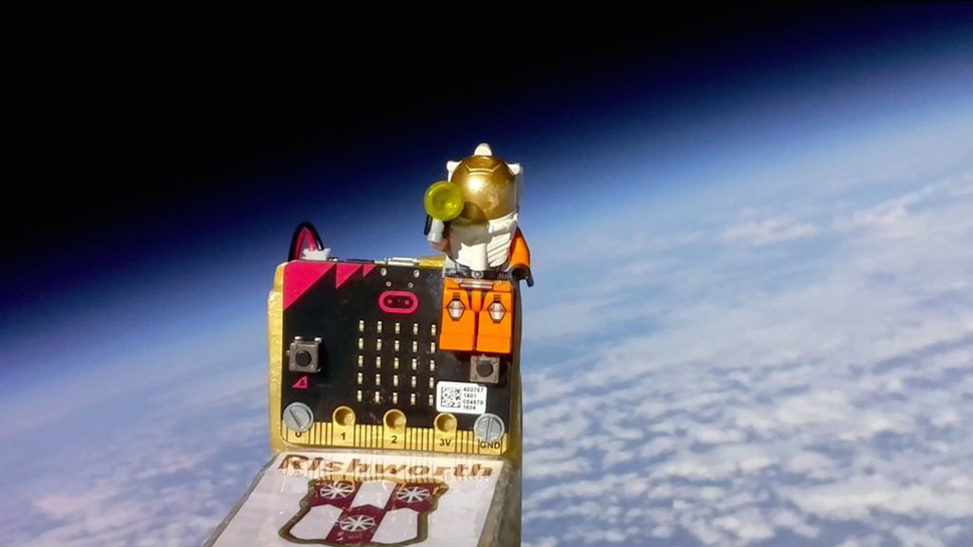
\includegraphics[width=.49\columnwidth] {images/microbit-space.jpg}
    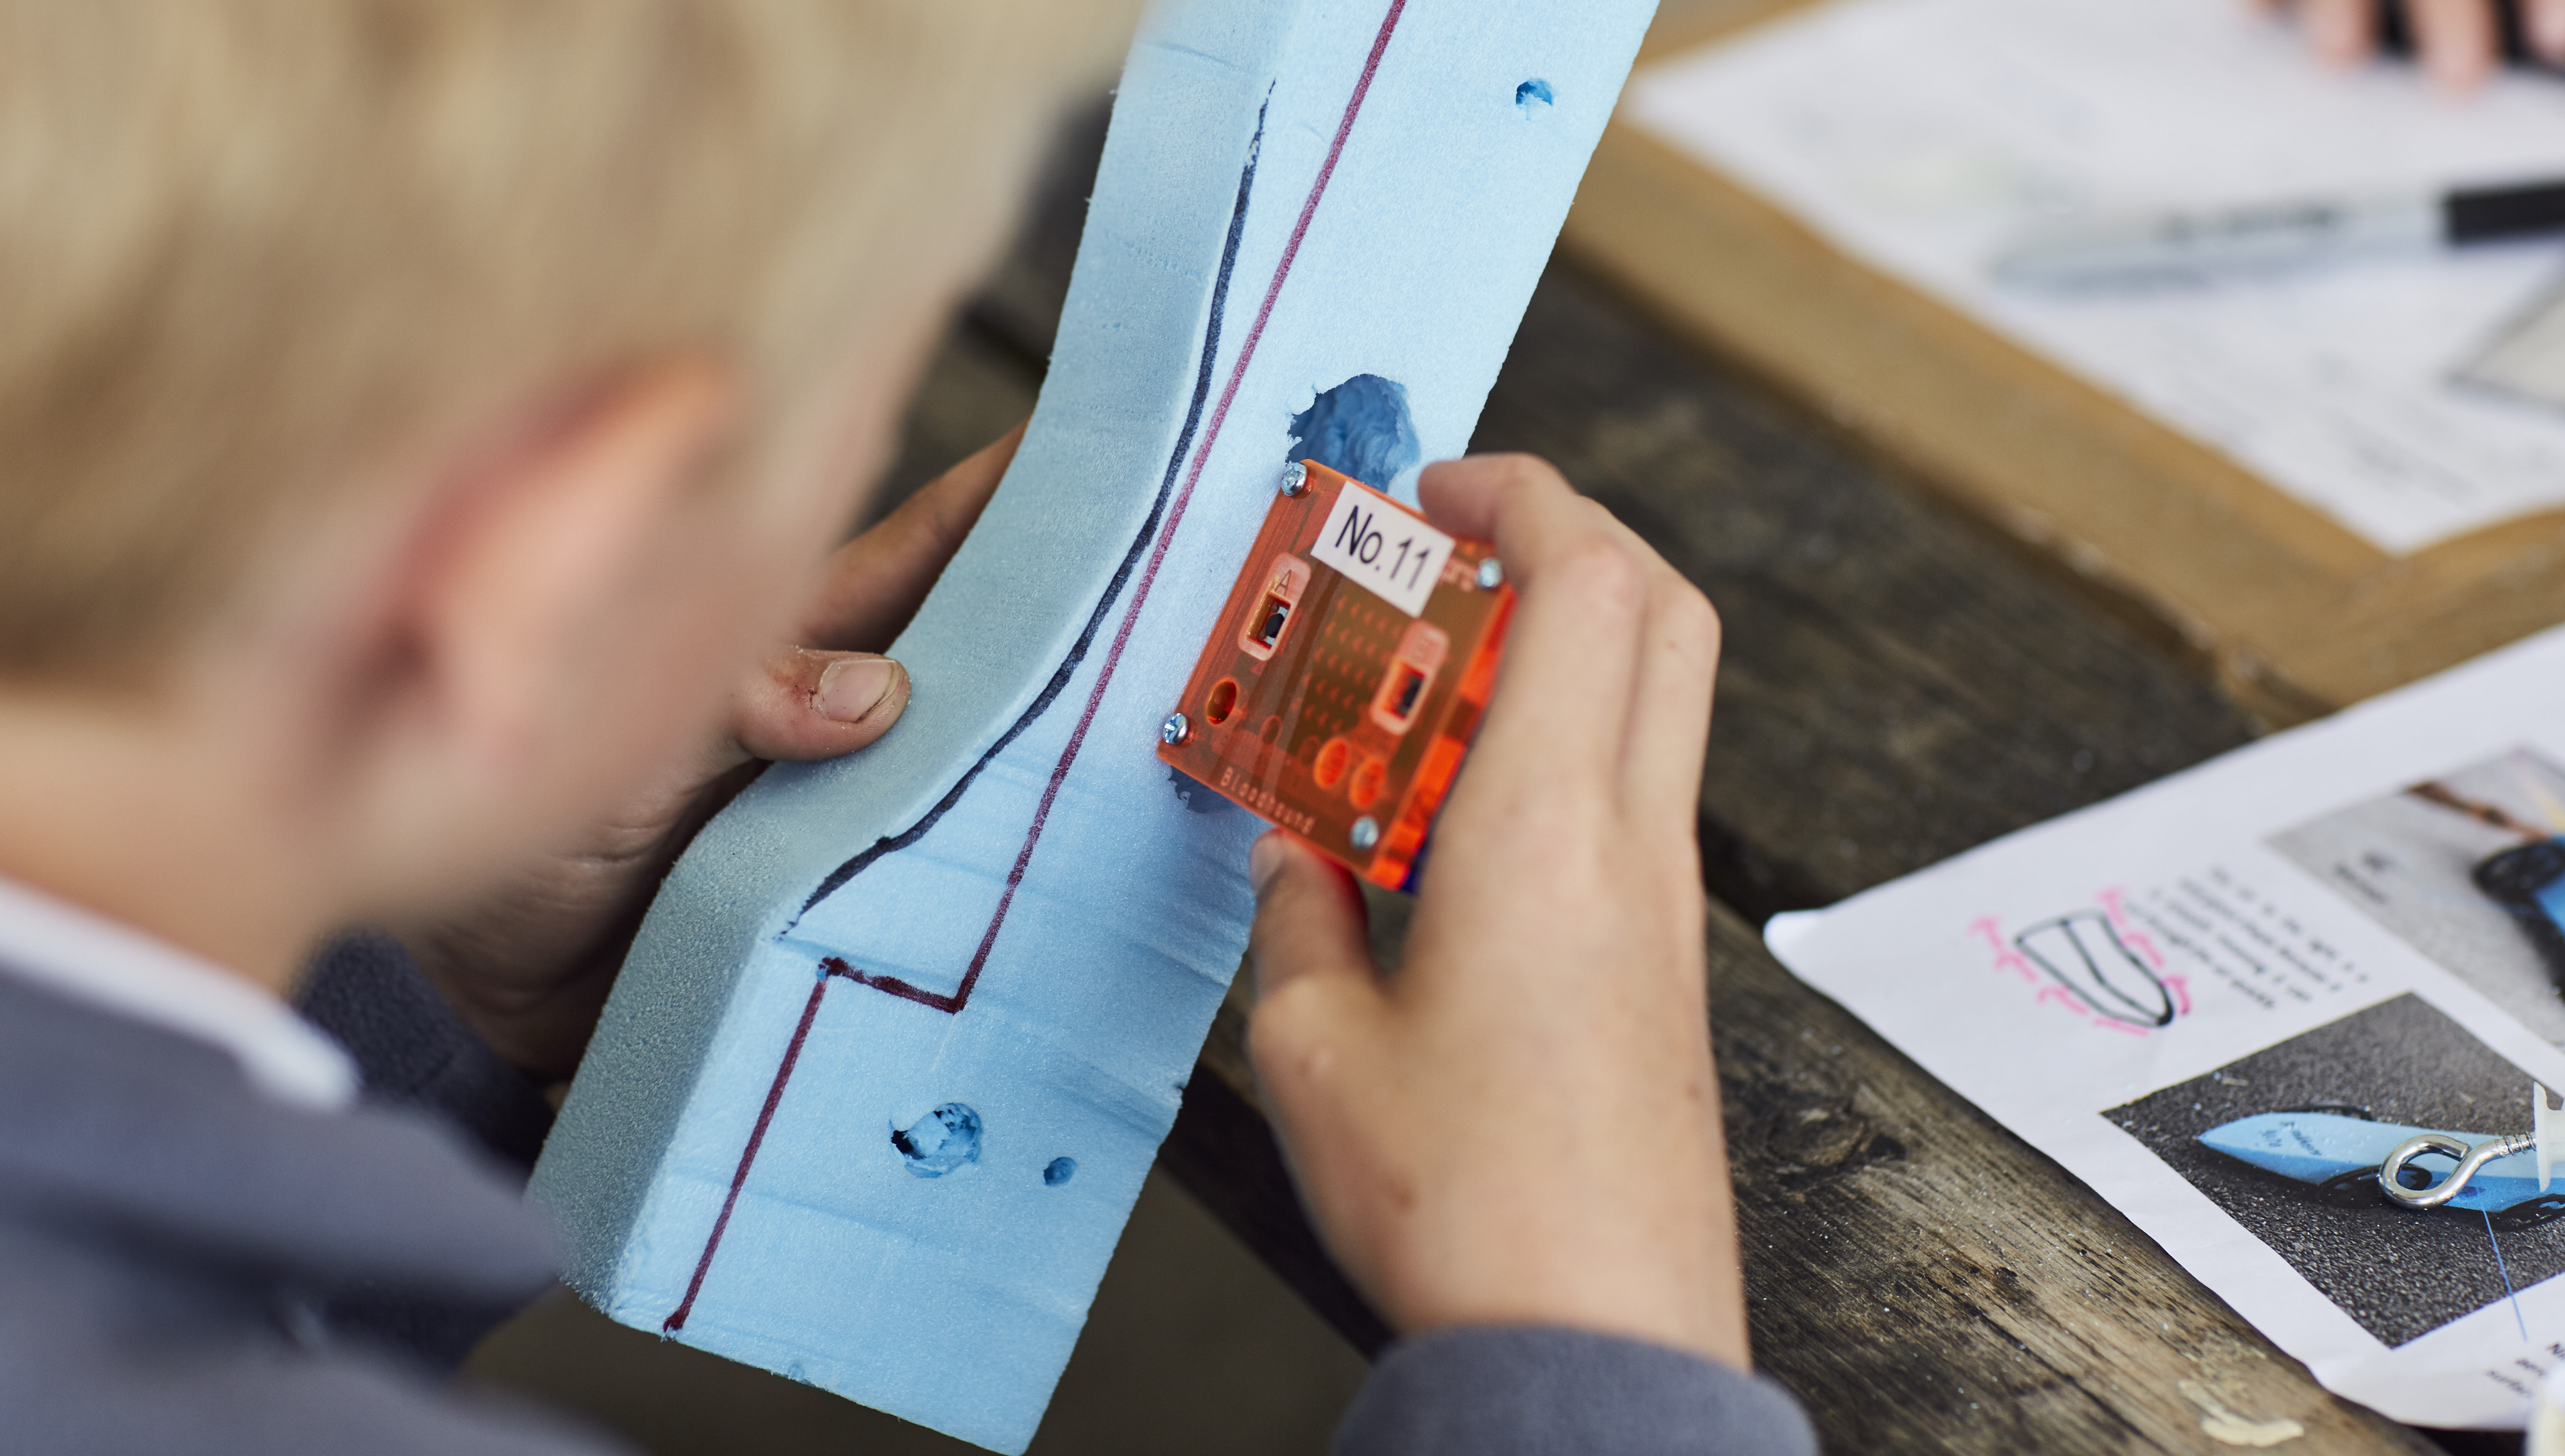
\includegraphics[width=.49\columnwidth]{images/bloodhound.jpg}
    \caption{\label{fig:projects} Example projects undertaken within education }
\end{figure}

Figure 1 highlights two example educational projects based on the BBC micro:bit. The first is a data gathering experiment, where multiple sensor data was recorded to non-volatile memory as the device was launched into near space (32.5km altitude), along with an externally interfaced camera and GPS unit. The second highlights a live data telemetry application, where acceleration data was streamed in real-time via Bluetooth Low Energy to enable the profiling of chemical-rocket powered model vehicles. These projects are highly sophisticated and were undertaken by high school educators and their students.

This paper introduces an open platform for embedded devices such as the micro:bit that enables the development of embedded applications by non-expert programmers. 

\subsection{Technical Considerations}
\label{sec:TechnicalChallenges}
Enabling novice programmers to succesfully develop embedded applications is a non-trivial task. During the course of our research we have identified a number of design challenges of this domain, that must be addressed by a succesful platform:

\paragraph{The Need For High Level Languages}
Programming languages for MCUs have not kept pace with advances in hardware and diversification of user domains. Despite active research in the field, the C/C++ languages remain the standard for embedded systems - and for good reasons: they provide a familiar imperative programming model, with compilers that produce highly efficient code, and enable low level access to hardware features when necessary. Popular examples include the Arduino project (\url{www.arduino.cc})~\cite{buildingArduino2014}, started in 2003, and ARM's Mbed platform (\url{www.mbed.org})~\cite{ARMmbed} --- both of which rely heavily on a C/C++ programming model. However, the limitations of using C/C++ as an application programming language for inexperienced developers are well understood~\cite{blikstein2013gears}. \emph{To address this, higher level languages like Python, JavaScript, and even visual programming langauges are required}. 

\paragraph{The Need For a Zero Installation Architecture}
The development environment for existing embedded systems typically requires the installation of complex (and often commercial) code editors, custom device drivers, compiler toolchains, and even additional programming hardware (such as a JLink programmer). For many (particularly in the field of education) this is an impossible task, due to the heterogeneity and policy constraints of their PCs. Often custom hardware and software is simply not permitted by policy and/or access to the necessary technical support. \emph{An effective solution must therefore provide a fully transparent, platform agnostic, zero installation experience to developing embedded software}.

\paragraph{Optimisation for Code Efficiency}
The domains described previously are enabled by small, highly resource-limited programmable embedded microcontrollers (or MCUs), which may have as little as a few kilobytes of RAM and FLASH memory.
Table~\ref{table:devices} compares the core capabilities of the class of MCU-based devices typically used in the education domain to a typical PC. Contrary to first impressions, these devices have a \emph{proportionally} large amount of processing power. 

\begin{table}[]
    \centering
    \begin{tabular}{|l|r|r|r|r|r|r|}
    \hline
                           &          &              & \bf{Word}  & \bf{CPU} &            \\
    \bf{Device}            & \bf{RAM} & \bf{Flash}   & \bf{Size}  & \bf{Speed} & \bf{CPU}  \\ \hline
    Uno            & 2 kB       & 32 kB      & 8          & 16MHz & AVR       \\ \hline
    micro:bit          & 16 kB      & 256 kB     & 32         & 16MHz & Cortex     \\ \hline
    CPX           & 32 kB      & 256 kB     & 32         & 48MHz & Cortex    \\ \hline
    PC             & 16 GB      & 1 TB       & 64         & 3GHz & Intel      \\ \hline
    \end{tabular}
    \caption{\label{table:devices}Example microcontroller devices in relationship to a typical PC. Device abbreviations: Uno (Arduino Uno), micro:bit (BBC micro:bit), CPX (Adafruit Circuit Playground Express); PC (Personal Computer).}
\end{table}

Consider the BBC micro:bit versus a typical PC. It has about 100 times less CPU power, but 10\textsuperscript{6} times less RAM, and 10\textsuperscript{6} times less storage. \emph{A language/runtime should therefore not only seek to provide high code density and spatial efficiency, but to actively trade off temporal efficiency for spatial efficiency where possible}.

\paragraph{Support for Asynchronous and Concurrent Programming} 
It is already well understood that novice programmers benefit from  event based programming paradigms. This is increasingly relevant when applied to embedded systems due to the typically asynchronous nature of the hardware. MCUs still follow Moore's law (the number of transistors doubles roughly every two years). However, this additional capacity is not typically invested in simply optimizing processing power. Instead, independent peripherals are integrated onto the same package as the CPU as a \emph{system-on-chip}. Examples  of such integrated hardware include Bluetooth/WiFi radio modules, audio inputs/outputs and simple graphical display hardware - all of which are capable of operating independently of the CPU. \emph{an effective language/runtime should directly support an asynchronous interaction model designed to cooperate with the independent nature of peripherals whilst remaining highly intuitive to the programmer}.

\paragraph{The Need for Intuitive and Extensible APIs} 
Intuitive APIs and programming models are required to support novice users, yet it is equally important that these APIs remain complete enough to realise the ambitious projects that are being undertaken by these communities. Providing simplicity through the reduction of functionality is not a valid approach. Also, embedded systems are becoming increasingly component based through wired and wireless interfaces such as I2C, Bluetooth Mesh, IEEE 802.15.4. \emph{An effective solution must therefore provide APIs that are consistent,  easy to understand and use, extensible to new hardware and also progressive such that their complexity grows with the capabilities of the programmer. }

\subsection{Paper Overview}
This paper focuses on the design, implementation, and evaluation of a new language, runtime and web-based development environment designed to address the above challenges for devices such as those listed in Table~\ref{table:devices}. Our results (Section~\ref{sec:evaluate}) show that these technologies combined can enable simplified programming through modern languages and event-based constructs while maintaining a relatively high degree of temporal and spatial efficiency. We demonstrate up to 50x better performance than other state-of-the-art implementations, in some cases nearing the performance of native C++.


% Our platform was deployed about a year ago at \url{www.makecode.com} and sees daily use by thousands of users.

% * Derive Requirements

% => Modern IoT Hardware
%     => Low cost
%     => 32 bit processor rich, ram poor MCUs
%     => Async h/ware

% => Universality

%   => Modern High level Langaguges
%     => Blocks
%     => Typescript
%     => C++
%     => Low barrier to entry
%     => Without sacrificing capability
%       => Temporal Efficiency
%       => Spacial Efficiency
%     => Async (HL languages are Async and the hardware is moving that way)
%     => First class Event support

%   => Modern Toolchains
%     => Universal Web based UI
%     => Driver free wired/wireless device integration

% * Paper Overview
% - background
%    - examples of awesomeness in the classroom, breaks the mould, not just blinking an LED
%    - scale
%    - non-trivial, engineering.
% - architecture
%    - makecode
%       - under the compiler section, mention no VM
%    - codal
%      - codal is not an RTOS
%    - uf2
% - eval
% - R/W
% - conclusions


% The emergence of a new breed of computer